\documentclass[10pt]{article}

\usepackage[T1]{fontenc}
\usepackage[utf8]{inputenc}
%\usepackage{beton}
%\usepackage{ccfonts}
%\usepackage{concrete}
\usepackage{concmath}
\usepackage{eulervm}
\usepackage{amsmath,amsthm,amssymb}
\usepackage{mathtools}
\usepackage{multicol}
\usepackage{marginnote}
\usepackage{pgfplots}
\usepackage{float}
\usepackage{hyperref}
\usepackage{bbm}
\usepackage{booktabs}
\usepackage{xcolor-solarized}
\usepackage{xcolor}
\pgfplotsset{compat=1.5}

\usepackage{listings}
\usepackage{xcolor}
\definecolor{codegreen}{rgb}{0,0.6,0}
\definecolor{codegray}{rgb}{0.5,0.5,0.5}
\definecolor{codepurple}{rgb}{0.58,0,0.82}
\definecolor{backcolour}{rgb}{0.95,0.95,0.92}
\lstdefinestyle{mystyle}{
    backgroundcolor=\color{backcolour},   
    commentstyle=\color{codegreen},
    keywordstyle=\color{magenta},
    numberstyle=\tiny\color{codegray},
    stringstyle=\color{codepurple},
    basicstyle=\ttfamily\footnotesize,
    breakatwhitespace=false,         
    breaklines=true,                 
    captionpos=b,                    
    keepspaces=true,                 
    numbers=left,                    
    numbersep=5pt,                  
    showspaces=false,                
    showstringspaces=false,
    showtabs=false,                  
    tabsize=2
}

\lstset{language=Python, style=mystyle}

\usepackage{mathtools}

\usepackage{wasysym}
\usepackage[margin=1.5in]{geometry} 
\usepackage{enumerate}
\index{\usepackage}\usepackage{multicol}

\newcommand{\N}{\mathbf{N}}
\newcommand{\Z}{\mathbb{Z}}

\newcommand{\R}{\mathbf{R}}
\newcommand{\C}{\mathbf{C}}
\newcommand{\Pbb}{\mathbb{P}}
\newcommand{\Fcal}{\mathcal{F}}
\newcommand{\Lcal}{\mathcal{L}}
\newcommand{\Acal}{\mathcal{A}}
\newcommand{\Ecal}{\mathcal{E}}
\newcommand{\Ebb}{\mathbb{E}}
\newcommand{\Qbb}{\mathbb{Q}}


\renewcommand{\mathbf}{\mathbold}

\newenvironment{theorem}[2][Theorem]{\begin{trivlist}
  \item[\hskip \labelsep {\bfseries #1}\hskip \labelsep {\bfseries #2.}]}{\end{trivlist}}
\newenvironment{lemma}[2][Lemma]{\begin{trivlist}
  \item[\hskip \labelsep {\bfseries #1}\hskip \labelsep {\bfseries #2.}]}{\end{trivlist}}
\newenvironment{exercise}[2][Exercise]{\begin{trivlist}
  \item[\hskip \labelsep {\bfseries #1}\hskip \labelsep {\bfseries #2.}]}{\end{trivlist}}
\newenvironment{reflection}[2][Reflection]{\begin{trivlist}
  \item[\hskip \labelsep {\bfseries #1}\hskip \labelsep {\bfseries #2.}]}{\end{trivlist}}
\newenvironment{proposition}[2][Proposition]{\begin{trivlist}
  \item[\hskip \labelsep {\bfseries #1}\hskip \labelsep {\bfseries #2.}]}{\end{trivlist}}
\newenvironment{corollary}[2][Corollary]{\begin{trivlist}
  \item[\hskip \labelsep {\bfseries #1}\hskip \labelsep {\bfseries #2.}]}{\end{trivlist}}

\newenvironment{definition}[2][Definition]{\begin{trivlist}
  \item[\hskip \labelsep {\bfseries #1}\hskip \labelsep {\bfseries #2.}]}{\end{trivlist}}

\definecolor{solar}{rgb}{0.9960, 0.9960, 0.9647}

\begin{document}
  \pagecolor{solar}
	
  \renewcommand{\qedsymbol}{\smiley}
	\title{Investments Class \\ Problem set 6}
	\author{Daniel Grosu, William Martin, Denis Steffen}
		
\maketitle

\begin{exercise}{1}
  \begin{itemize}
    \item We can first compute the expected stock return using the formula of the model, and we obtain by linearity of the expectation: 
     $$ \Ebb[R_i] = \alpha_i + \sum_{k=1}^K B_{ik}\Ebb[F_k] + \Ebb[\epsilon_i] = \alpha_i + \sum_{k=1}^K B_{ik}m_k $$
     The Arbitrage Pricing Theory requires that the expected stock return has the following form: $$ \Ebb[R_i] = R_0 + \sum_{k=1}^K B_{ik}m_k^e$$ where $m_k^e$ are the expected excess returns ($m_k^e = m_k - R_0$). 
     So, we obtain the condition for $\alpha_i$: 
     $$ \alpha_i = R_0 - R_0\sum_{k=1}^K B_{ik} = R_0(1-\sum_{k=1}^KB_{ik})$$
    \item If the market portfolio is spanned by the factors, we have $$ R_M = \sum_{k=1}^Kw_kF_k$$ And the CPAM holds if $$ \Ebb[R_i] = R_0 + \beta_i(\Ebb[R_M]-R_0) = R_0 + \frac{Cov(R_i,R_M)}{\sigma_M^2}(\sum_{k=1}^Kw_km_k-R_0)$$
    $$ = R_0 + \left(\frac{1}{\sigma_M^2}\sum_{k=1}^KB_{ik}Cov(F_k,R_M)\right)(\sum_{k=1}^Kw_km_k-R_0)$$ because the $(F_k)_{1\leq k\leq K}$ random variables are independent.
    \\
    So, we can rewrite the expectation using $\beta_{F_k} = \frac{Cov(F_k,R_M)}{\sigma_M^2}$ as: 
    \begin{align*}
      \Ebb[R_i] &= R_0 + \left(\sum_{k=1}^K B_{ik}\beta_{F_k}\right)\left(\sum_{k=1}^Kw_km_k-R_0\right) \\
      &= R_0 + \sum_{k=1}^K B_{ik}(\beta_{F_k}(\Ebb[R_M]-R_0)) \\
      &= R_0 + \sum_{k=1}^K B_{ik}\lambda_k
    \end{align*} where $ \lambda_k = \beta_{F_k}(\Ebb[R_M]-R_0) = \Ebb[F_k] - R_0$, by the CPAM relation for $F_k$.

    Thus, we know that the APT must hold: 
    $$ \Ebb[R_i] = R_0 + \sum_{k=1}^K B_{ik}(\Ebb[F_k] - R_0) = R_0 + \sum_{k=1}^K B_{ik}(m_k^e)$$ and this is true if and only if the CPAM holds.
    We need to have: $$ \beta_{F_k}(\sum_{l=1}^K w_lm_l - R_0) = m_k - R_0$$ and so $$ \sum_{l=1}^K w_lm_l = R_0 + \frac{m_k-R_0}{\beta_{F_k}}\quad \text{(risk premia)}$$
    and $$ \sigma_M^2 = \sum_{k=1}^K w_k^2(\sigma_k^2 + m_k^2)-(\sum_{k=1}^Kw_km_k)^2 \quad \text{(volatility)}$$
    \item In this case we have that: 
    $$ \Ebb[R_i] = R_0 + \sum_{k=1}^K B_{ik}\lambda_k$$ and so for $N$ assets in portfolio $p$:
    $$ \Ebb[R_p] = \frac{1}{N}\sum_{i=1}^N\Ebb[R_i] = \frac{1}{N}\sum_{i=1}^N(R_0 + \sum_{k=1}^K B_{ik}\lambda_k)$$, using that $B_{ik}\geq b \forall (i,k)$
    $$ \Ebb[R_p] \geq \frac{1}{N}\left(NR_0 + N\sum_{k=1}^K b\lambda_k\right) = R_0 + b\sum_{k=1}^K\lambda_k > 0 $$ because $b> 0, \lambda_k >0 \text{ and } R_0 \geq 0$.

    Hence, we see that the returns do not converge to zero when the number of assets $N$ tends to infinity. This contradicts the Arbitrage Pricing Theory on fully diversified portfolios that requires $ \frac{1}{N}\sum_{i=1}^Nw_i\nu_i \rightarrow 0$ when $N \rightarrow \infty$.  

    We can see that the volatility of each asset is $V(R_i) = \sigma_{\epsilon}$ because $\sum_{k=1}^KB_{ik}\lambda_k$ is deterministic and known. 
    So for the portfolio: 
    $$ V(R_p) = \frac{1}{N^2}\sum_{i=1}^N\sigma_{\epsilon} = \frac{1}{N}\sigma_\epsilon \rightarrow 0 \quad \text{when } N \rightarrow \infty$$
    So the asymptotic arbitrage portfolio is given by $w = (\pm\frac{1}{N},\dots,\pm\frac{1}{N})$ such that $\mathbbm{1}'w = 0$. If $N$ is even, it suffices to short the half of the assets and long the other half. If $N$ is odd, we can choose $w = (+\frac{1}{N},-\frac{1}{N},\dots,+\frac{1}{N},-\frac{1}{2N},-\frac{1}{2N})$.
    This portfolio has stricly positive expected profits (as $\Ebb[R_p] > 0$) and no risk (as $V(R_p)\rightarrow 0$) without initial investment. We have an asymptotic artbitrage portfolio. 
  \end{itemize}
	
\end{exercise}

\begin{exercies}{2}
  In the following discussion we will refer to the \textit{full sample} as the
  stock returns data of the 636 stocks from 2000-01-31 to 2019-12-31, the
  \textit{first sample} as the subsample from 2000-01-31 to 2009-12-31 and the
  \textit{second sample} as the subsample from 2010-01-31 to 2019-12-31. In the
  figure below we plot the excess returns against beta of the portfolios corresponding to 
  the $0-10, 10-20, 20-30, \ldots, 90-100$ market beta quantiles of stocks. The excess
  returns and the betas are empirically estimated over the full sample.

  \begin{figure}[H]
    \centering
    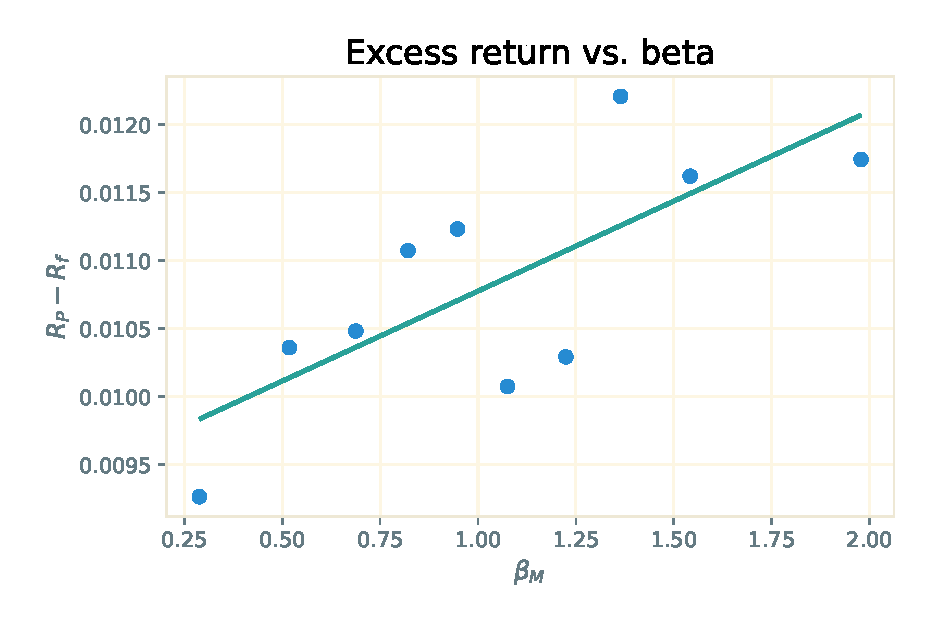
\includegraphics[width=0.7\linewidth]{plot1.eps}
    \caption{Excess return against beta: full sample.}
  \end{figure}

  It is clearly observed that the risk-premium is significant over the
  full-sample: high-beta portfolios achieve higher returns.

  \begin{figure}[H]
    \centering
    \includegraphics[width=0.7\linewidth]{plot2.eps}
    \caption{Excess return against beta: first sample portfolios with second
      sample market returns.}
  \end{figure}

  If one computes the portfolios based on the first subsample and keeps them
  static over the second sample, the correlations between high beta and higher
  return is not clearly observed: the fitted line is mostly flat. Why? Perhaps
  over the decade, the portfolios have changed their sensitivity to the market
  and the market has incorporated quickly information, offering an either higher
  or lower risk premium than previously awarded. In the language that we used in
  the class, the high and low beta portfolios do not have much
  \textit{beta-}momentum from the first to the second decade of the twenty-first
  century.

  Theoretically, the beta of the market is $\beta_M = 1$. Hence, to test whether
  the CAPM holds for the full sample, we can evaluate $r_M = 1 \times a$ where a
  is the slope of the empirical SML line and check whether their difference is
  close to zero. The slope of the fitted line is: $a=0.00132$ and the average
  excess market retun over the risk-free rate is $r_M - r_f = 0.00451$ monthly. Clearly,
  this shows that CAPM does not fully explain the market and that there are
  other factors and sources of risk which are not priced in the current model.

  However, there is another explanation. In the table below we provide the betas
  of the decile portfolios in the first sample and the betas of the same
  portfolios in the second sample:
  \begin{table}[H]
    \centering
    \begin{tabular}{| c | c | c |}
      \hline\hline
      Quantile & 2000-2009 & 2010-2019 \\ \hline \hline
1.0       &       0.219238    &     0.539616 \\ \hline
2.0        &      0.412684    &     0.757070 \\ \hline
3.0         &     0.573625    &     0.929977 \\ \hline
4.0         &     0.715312    &     1.052507 \\ \hline
5.0         &     0.842216    &     1.207823 \\ \hline
6.0         &     0.961448    &     1.284644 \\ \hline
7.0         &     1.139001    &     1.392084 \\ \hline
8.0         &     1.330552    &     1.475634 \\ \hline
9.0         &     1.576502    &     1.490454 \\ \hline
10.0         &     2.041873    &     1.782677 \\ \hline
    \end{tabular}
    \caption{Betas of the static portfolios during 2000-2009 and 2010-2019}
  \end{table}


  The ``regression to the mean'' phenomena is clearly visible: the low beta
  portfolios become larger beta portfolios and the high beta portfolios become
  smaller beta portfolios. Although this phenomena can be explained with a
  purely probabilistic argument: that the extreme events in a first draw have the
  highest probability of during the second draw around the mean, we think there
  is more to this phenomena than just randomness, because the performance of
  equities are at the end of the day tied to the fundamentals of the firm. The
  low-beta portfolios formed out of stocks of firms with less sensitivity to the
  market increase in their sensitivity because of the globalization and the
  interconnectedness between firms that has increased over the second decade.
  The high beta portfolios with stocks of firms with high sensitivity (also
  smaller firms), grow in their size and establish themselves, leading to less
  risky cash flows and hence less sensitivity. This phenomena can also be a
  consequence of the investment sentiment in the wake of the 2008 financial
  crisis: the preference of the investors has tilted towards less risky
  equities and companies undertook less risky projects because they were not
  compensated by the investors for the extra risk in their cash flows.

  

  \begin{figure}[H]
    \centering
    \includegraphics[width=0.7\linewidth]{plot3.eps}
    \caption{First beta portfolios against second beta portfolios.}
  \end{figure}
\end{exercise}
  
\end{document}


\section{Appendix}
\lstinputlisting[language=Python]{ps6_py.py}
\appendix
